\documentclass[a4paper,11pt]{report}
\usepackage{chuan_math_gkt}
\usetikzlibrary{angles,quotes,intersections,patterns,decorations.pathreplacing}
\chuanexamsetup

\begin{document}
\examfontsize

\examsecret{绝密$\bigstar$启用前}

\examtitle{2021年普通高等学校招生全国统一考试（北京卷）}{数\quad 学}

\noticetitle
\begin{examnotice}
\item 答卷前，考生务必将自己的姓名、准考证号填写在答题卡上. 
\item 回答选择题时，选出每小题的答案后，用铅笔把答题卡上对应题目的答案标号涂黑. 如需改动，用橡皮擦干净后，再选涂其他答案标号. 回答非选择题时，将答案写在答题卡上. 写在本试卷上无效. 
\item 考试结束后，将本试卷和答题卡一并交回. 
\end{examnotice}


\examsection{一、选择题：本题共10小题，每小题4分，共40分. 在每小题给出的四个选项中，只有一项是符合题目要求的. }
\begin{examquestions}
\item 已知集合 $A=\{x\mid -1<x<1\}$，$B=\{x\mid 0\leq x\leq2\}$，则 $A\cup B=$
\fourchoices{$(-1,2)$}{$(-1,2]$}{$[0,1)$}{$[0,1]$}
\item 在复平面内，复数 $z$ 满足 $(1-\mathrm{i})z=2$，则 $z=$
\fourchoices{$2+\mathrm{i}$}{$2-\mathrm{i}$}{$1-\mathrm{i}$}{$1+\mathrm{i}$}
\item 已知 $f(x)$ 是定义在 $[0,1]$ 上的函数，那么“函数 $f(x)$ 在 $[0,1]$ 上单调递增”是“函数 $f(x)$ 在 $[0,1]$ 上的最大值为 $f(1)$”的
\twochoices{充分而不必要条件}{必要而不充分条件}{充分必要条件}{既不充分也不必要条件}
\item 某四面体的三视图如图所示，该四面体的表面积为
\fourchoices{$\dfrac{3+\sqrt3}{2}$}{$4$}{$3+\sqrt3$}{$2$}
\begin{tightcenter}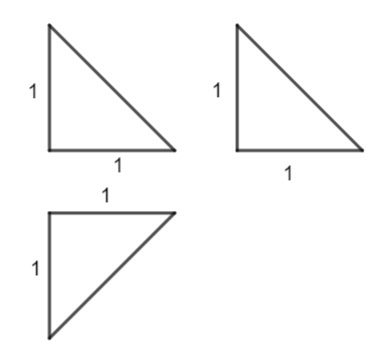
\includegraphics[width=4cm]{figures/2021_bj_q4.png}\end{tightcenter}
\item 双曲线 $C:\dfrac{x^2}{a^2}-\dfrac{y^2}{b^2}=1$ 过点 $(\sqrt2,\sqrt3)$，且离心率为 $2$，则该双曲线的标准方程为
\fourchoices{$x^2-\dfrac{y^2}{3}=1$}{$\dfrac{x^2}{3}-y^2=1$}{$x^2-\dfrac{\sqrt3y^2}{3}=1$}{$\dfrac{\sqrt3x^2}{3}-y^2=1$}
\item $\{a_n\}$ 和 $\{b_n\}$ 是两个等差数列，其中 $\dfrac{a_k}{b_k}(1\leq k\leq5)$ 为常值，$a_1=288$，$a_5=96$，$b_1=192$，则 $b_3=$
\fourchoices{$64$}{$128$}{$256$}{$512$}
\item 函数 $f(x)=\cos x-\cos 2x$，试判断函数的奇偶性及最大值
\twochoices{奇函数，最大值为 $2$}{偶函数，最大值为 $2$}{奇函数，最大值为 $\dfrac98$}{偶函数，最大值为 $\dfrac98$}
\noindent\begin{minipage}[t]{0.75\linewidth}
\item 定义：$24$ 小时内降水在平地上积水厚度（$\mathrm{mm}$）来判断降雨程度. 其中小雨（$<10\mathrm{mm}$），中雨（$10\mathrm{mm}\sim25\mathrm{mm}$），大雨（$25\mathrm{mm}\sim50\mathrm{mm}$），暴雨（$50\mathrm{mm}\sim100\mathrm{mm}$）. 小明用一个圆锥形容器接了 $24$ 小时雨水，如图，则这天降雨属于哪个等级
\vspace{0.5em}
\twochoices{小雨}{中雨}{大雨}{暴雨}
\end{minipage}\hfill
\begin{minipage}[t]{0.21\linewidth}
\vspace{0em}\centering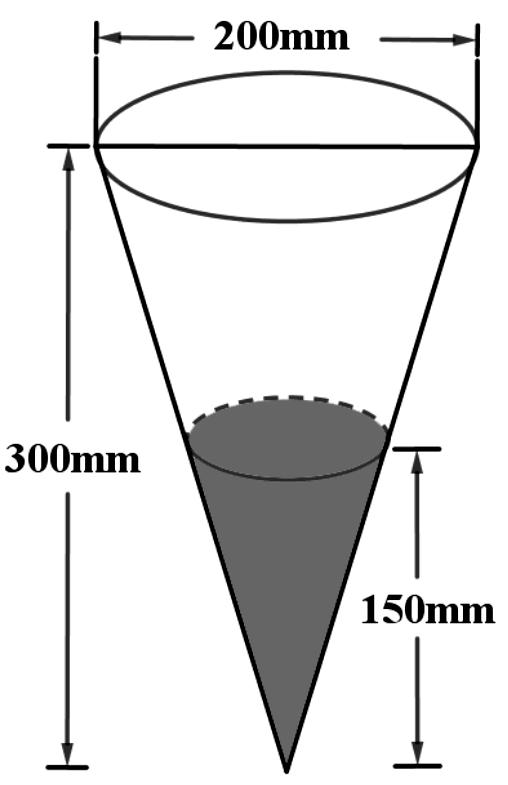
\includegraphics[width=\linewidth]{figures/2021_bj_q8.png}
\end{minipage}
\item 已知圆 $C:x^2+y^2=4$，直线 $l:y=kx+m$，当 $k$ 变化时，$l$ 截得圆 $C$ 弦长的最小值为 $2$，则 $m=$
\fourchoices{$\pm2$}{$\pm\sqrt2$}{$\pm\sqrt3$}{$\pm\sqrt5$}
\item 数列 $\{a_n\}$ 是递增的整数数列，且 $a_1\geq3$，$a_1+a_2+\cdots+a_n=100$，则 $n$ 的最大值为
\fourchoices{$9$}{$10$}{$11$}{$12$}
\end{examquestions}

\examsection{二、填空题：本题共5小题，每小题5分，共25分. }
\begin{examquestions}[start=11]
\item $(x^3-\dfrac1x)^4$ 展开式中常数项为\blank.
\item 已知抛物线 $C:y^2=4x$，焦点为 $F$，点 $M$ 为抛物线 $C$ 上的点，且 $|FM|=6$，则 $M$ 的横坐标是\blank；作 $MN\perp x$ 轴于 $N$，则 $S_{\triangle FMN}=$\blank.
\item $\vec a=(2,1)$，$\vec b=(2,-1)$，$\vec c=(0,1)$，则 $(\vec a+\vec b)\cdot\vec c=$\blank；$\vec a\cdot\vec b=$\blank.
\item 若点 $P(\cos\theta,\sin\theta)$ 与点 $Q(\cos(\theta+\dfrac\pi6),\sin(\theta+\dfrac\pi6))$ 关于 $y$ 轴对称，写出一个符合题意的 $\theta=$\blank.
\item 已知函数 $f(x)=\lg|x|-kx-2$，给出下列四个结论：①若 $k=0$，则 $f(x)$ 有两个零点；②$\exists k<0$，使得 $f(x)$ 有一个零点；③$\exists k<0$，使得 $f(x)$ 有三个零点；④$\exists k>0$，使得 $f(x)$ 有三个零点. 以上正确结论序号是\blank.
\end{examquestions}
\newpage
\examsection{三、解答题：本题共6小题，共85分. 解答应写出文字说明、证明过程或演算步骤. }
\begin{examanswers}[start=16]
\item（13分）

已知 $\triangle ABC$ 中，$c=2b\cos B$，$C=\dfrac{2\pi}{3}$.

\subq{（1）}{求 $B$ 的大小；}

\subq{（2）}{在下列三个条件中选择一个作为已知，使 $\triangle ABC$ 存在且唯一确定，并求出 $BC$ 边上的中线的长度. 

条件①：$c=\sqrt2 b$；

条件②：周长为 $4+2\sqrt3$；

条件③：面积为 $S_{\triangle ABC}=\dfrac{3\sqrt3}{4}$.}
\item（13分）

已知正方体 $ABCD-A_1B_1C_1D_1$，点 $E$ 为 $A_1D_1$ 中点，直线 $B_1C$ 交平面 $CDE$ 于点 $F$.

\noindent\begin{minipage}[t]{0.6\linewidth}
\subq{（1）}{证明：点 $F$ 为 $B_1C$ 的中点；}

\subq{（2）}{若点 $M$ 为棱 $A_1B_1$ 上一点，且二面角 $M-CF-E$ 的余弦值为 $\dfrac{\sqrt5}{3}$，求 $\dfrac{A_1M}{A_1B_1}$ 的值.}
\end{minipage}\hfill
\begin{minipage}[t]{0.35\linewidth}
\vspace{0em}\centering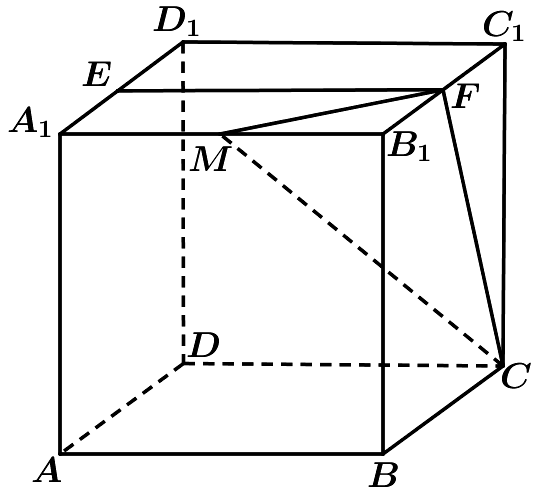
\includegraphics[width=\linewidth]{figures/2021_bj_q17.png}
\end{minipage}
\item（14分）

为加快新冠肺炎检测效率，某检测机构采取“$k$ 合 $1$ 检测法”，即将 $k$ 个人的拭子样本合并检测，若为阴性，则可以确定所有样本都是阴性的；若为阳性，则还需要对本组的每个人再做检测. 现有 $100$ 人，已知其中 $2$ 人感染病毒.

\subq{（1）}{}

\subq{（i）}{若采用“$10$ 合 $1$ 检测法”，且两名患者在同一组，求总检测次数；}

\subq{（ii）}{已知 $10$ 人分成一组，分 $10$ 组，两名感染患者在同一组的概率为 $\dfrac1{11}$，定义随机变量 $X$ 为总检测次数，求检测次数 $X$ 的分布列和数学期望 $E(X)$；}


\subq{（2）}{若采用“$5$ 合 $1$ 检测法”，检测次数 $Y$ 的期望为 $E(Y)$，试比较 $E(X)$ 和 $E(Y)$ 的大小（直接写出结果）.\newpage}
\item（15分）

已知函数 $f(x)=\dfrac{3-2x}{x^2+a}$.

\subq{（1）}{若 $a=0$，求 $y=f(x)$ 在 $(1,f(1))$ 处切线方程；}

\subq{（2）}{若函数 $f(x)$ 在 $x=-1$ 处取得极值，求 $f(x)$ 的单调区间，以及最大值和最小值.}
\item（15分）

已知椭圆 $E:\dfrac{x^2}{a^2}+\dfrac{y^2}{b^2}=1(a>b>0)$ 过点 $A(0,-2)$，以四个顶点围成的四边形面积为 $4\sqrt5$.

\subq{（1）}{求椭圆 $E$ 的标准方程；}

\subq{（2）}{过点 $P(0,-3)$ 的直线 $l$ 斜率为 $k$，交椭圆 $E$ 于不同的两点 $B$，$C$，直线 $AB$，$AC$ 分别交 $y=-3$ 于点 $M$，$N$，若 $|PM|+|PN|\leq15$，求 $k$ 的取值范围.}
\item（15分）

定义 $R_p$ 数列 $\{a_n\}$：对实数 $p$，满足：① $a_1+p\geq0$，$a_2+p=0$；② $\forall n\in\mathbb N^*$，$a_{4n-1}<a_{4n}$；③ $a_{m+n}\in[a_m+a_n+p,a_m+a_n+p+1]$，$m,n\in\mathbb N^*$.

\subq{（1）}{对于前 $4$ 项 $2,-2,0,1$ 的数列，可以是 $R_2$ 数列吗？说明理由；}

\subq{（2）}{若 $\{a_n\}$ 是 $R_0$ 数列，求 $a_5$ 的值；}

\subq{（3）}{是否存在 $p$，使得存在 $R_p$ 数列 $\{a_n\}$，对 $\forall n\in\mathbb N^*$，$S_n\geq S_{10}$？若存在，求出所有这样的 $p$；若不存在，说明理由.}
\end{examanswers}

\end{document}
